
\documentclass[11pt,compress,t,notes=noshow, xcolor=table]{beamer}
\usepackage[]{graphicx}\usepackage[]{color}
% maxwidth is the original width if it is less than linewidth
% otherwise use linewidth (to make sure the graphics do not exceed the margin)
\makeatletter
\def\maxwidth{ %
  \ifdim\Gin@nat@width>\linewidth
    \linewidth
  \else
    \Gin@nat@width
  \fi
}
\makeatother

\definecolor{fgcolor}{rgb}{0.345, 0.345, 0.345}
\newcommand{\hlnum}[1]{\textcolor[rgb]{0.686,0.059,0.569}{#1}}%
\newcommand{\hlstr}[1]{\textcolor[rgb]{0.192,0.494,0.8}{#1}}%
\newcommand{\hlcom}[1]{\textcolor[rgb]{0.678,0.584,0.686}{\textit{#1}}}%
\newcommand{\hlopt}[1]{\textcolor[rgb]{0,0,0}{#1}}%
\newcommand{\hlstd}[1]{\textcolor[rgb]{0.345,0.345,0.345}{#1}}%
\newcommand{\hlkwa}[1]{\textcolor[rgb]{0.161,0.373,0.58}{\textbf{#1}}}%
\newcommand{\hlkwb}[1]{\textcolor[rgb]{0.69,0.353,0.396}{#1}}%
\newcommand{\hlkwc}[1]{\textcolor[rgb]{0.333,0.667,0.333}{#1}}%
\newcommand{\hlkwd}[1]{\textcolor[rgb]{0.737,0.353,0.396}{\textbf{#1}}}%
\let\hlipl\hlkwb

\usepackage{framed}
\makeatletter
\newenvironment{kframe}{%
 \def\at@end@of@kframe{}%
 \ifinner\ifhmode%
  \def\at@end@of@kframe{\end{minipage}}%
  \begin{minipage}{\columnwidth}%
 \fi\fi%
 \def\FrameCommand##1{\hskip\@totalleftmargin \hskip-\fboxsep
 \colorbox{shadecolor}{##1}\hskip-\fboxsep
     % There is no \\@totalrightmargin, so:
     \hskip-\linewidth \hskip-\@totalleftmargin \hskip\columnwidth}%
 \MakeFramed {\advance\hsize-\width
   \@totalleftmargin\z@ \linewidth\hsize
   \@setminipage}}%
 {\par\unskip\endMakeFramed%
 \at@end@of@kframe}
\makeatother

\definecolor{shadecolor}{rgb}{.97, .97, .97}
\definecolor{messagecolor}{rgb}{0, 0, 0}
\definecolor{warningcolor}{rgb}{1, 0, 1}
\definecolor{errorcolor}{rgb}{1, 0, 0}
\newenvironment{knitrout}{}{} % an empty environment to be redefined in TeX

\usepackage{alltt}
\newcommand{\SweaveOpts}[1]{}  % do not interfere with LaTeX
\newcommand{\SweaveInput}[1]{} % because they are not real TeX commands
\newcommand{\Sexpr}[1]{}       % will only be parsed by R
\newcommand{\xmark}{\ding{55}}%


\usepackage[english]{babel}
\usepackage[utf8]{inputenc}

\usepackage{dsfont}
\usepackage{verbatim}
\usepackage{amsmath}
\usepackage{amsfonts}
\usepackage{amssymb}
\usepackage{bm}
\usepackage{csquotes}
\usepackage{multirow}
\usepackage{longtable}
\usepackage{booktabs}
\usepackage{enumerate}
\usepackage[absolute,overlay]{textpos}
\usepackage{psfrag}
\usepackage{algorithm}
\usepackage{algpseudocode}
\usepackage{eqnarray}
\usepackage{arydshln}
\usepackage{tabularx}
\usepackage{placeins}
\usepackage{tikz}
\usepackage{setspace}
\usepackage{colortbl}
\usepackage{mathtools}
\usepackage{wrapfig}
\usepackage{bm}
\usepackage{amsmath}
\usepackage{pifont}
\usepackage{xcolor} %colored math symbols

\usetikzlibrary{shapes,arrows,automata,positioning,calc,chains,trees, shadows}
\tikzset{
  %Define standard arrow tip
  >=stealth',
  %Define style for boxes
  punkt/.style={
    rectangle,
    rounded corners,
    draw=black, very thick,
    text width=6.5em,
    minimum height=2em,
    text centered},
  % Define arrow style
  pil/.style={
    ->,
    thick,
    shorten <=2pt,
    shorten >=2pt,}
}

\usepackage{subfig}

% Defines macros and environments
\usepackage{../../style/lmu-lecture}


\let\code=\texttt
\let\proglang=\textsf

\setkeys{Gin}{width=0.9\textwidth}

\setbeamertemplate{frametitle}{\expandafter\uppercase\expandafter\insertframetitle}

\usepackage{bbm}
% basic latex stuff
\newcommand{\pkg}[1]{{\fontseries{b}\selectfont #1}} %fontstyle for R packages
\newcommand{\lz}{\vspace{0.5cm}} %vertical space
\newcommand{\dlz}{\vspace{1cm}} %double vertical space
\newcommand{\oneliner}[1] % Oneliner for important statements
{\begin{block}{}\begin{center}\begin{Large}#1\end{Large}\end{center}\end{block}}


%new environments
\newenvironment{vbframe}  %frame with breaks and verbatim
{
 \begin{frame}[containsverbatim,allowframebreaks]
}
{
\end{frame}
}

\newenvironment{vframe}  %frame with verbatim without breaks (to avoid numbering one slided frames)
{
 \begin{frame}[containsverbatim]
}
{
\end{frame}
}

\newenvironment{blocki}[1]   % itemize block
{
 \begin{block}{#1}\begin{itemize}
}
{
\end{itemize}\end{block}
}

\newenvironment{fragileframe}[2]{  %fragile frame with framebreaks
\begin{frame}[allowframebreaks, fragile, environment = fragileframe]
\frametitle{#1}
#2}
{\end{frame}}


\newcommand{\myframe}[2]{  %short for frame with framebreaks
\begin{frame}[allowframebreaks]
\frametitle{#1}
#2
\end{frame}}

\newcommand{\remark}[1]{
  \textbf{Remark:} #1
}


\newenvironment{deleteframe}
{
\begingroup
\usebackgroundtemplate{
\includegraphics[width=\paperwidth,height=\paperheight]{../style/color/red.png}}
 \begin{frame}
}
{
\end{frame}
\endgroup
}
\newenvironment{simplifyframe}
{
\begingroup
\usebackgroundtemplate{
\includegraphics[width=\paperwidth,height=\paperheight]{../style/color/yellow.png}}
 \begin{frame}
}
{
\end{frame}
\endgroup
}\newenvironment{draftframe}
{
\begingroup
\usebackgroundtemplate{
\includegraphics[width=\paperwidth,height=\paperheight]{../style/color/green.jpg}}
 \begin{frame}
}
{
\end{frame}
\endgroup
}
% https://tex.stackexchange.com/a/261480: textcolor that works in mathmode
\makeatletter
\renewcommand*{\@textcolor}[3]{%
  \protect\leavevmode
  \begingroup
    \color#1{#2}#3%
  \endgroup
}
\makeatother


\input{../../latex-math/basic-math}
\input{../../latex-math/basic-ml}
\input{../../latex-math/ml-nn}

\newcommand{\titlefigure}{plots/05_conv_variations/separable/Depthwise.png}
%modify picture
\newcommand{\learninggoals}{
  \item Separable Convolutions
  \item Flattening
}

\title{Deep Learning}
\date{}



\begin{document}

\lecturechapter{Separable Convolutions and Flattening}
\lecture{I2DL}

%%%%%%%%%%%%%%%%%%%%%%%%%%%%%%%%%%%%%%%%

%%%%%%%%%%%%%%%%%%%%%%%%%%%%%%%%%%%%%%%%
%%%%%%%%%%%%%%%%%%%%%%%%%%%%%%%%%%%%%%%%%%%

\section{Separable Convolutions}

 \begin{vbframe}{Separable convolutions}
     \begin{itemize}
         \item Separable Convolutions are used in some neural net architectures, such as the MobileNet.
         \item Motivation: make convolution computationally more efficient.
         \item One can perform:
               \begin{itemize}
                   \item spatially separable convolution 
                   \item depthwise separable convolution.
                \end{itemize}
      \end{itemize}
      The \textbf{spatially separable convolution} operates on the 2D spatial dimensions of images, i.e. height and width. Conceptually, spatially separable convolution decomposes a convolution into two separate operations.
      \begin{itemize}   
         \item Consider the sobel kernel from the previous lecture:
             \begin{equation*}
                     G_x = 
                     \begin{bmatrix}
                         +1 & 0 & -1 \\
                         +2 & 0 & -2 \\
                         +1 & 0 & -1 
                     \end{bmatrix}
             \end{equation*}
         \item this 3x3 dimensional kernel can be replaced by the outer product of two 3x1 and 1x3 dimensional kernels:
            \begin{equation*}
                     \begin{bmatrix}
                         +1 \\ 
                         +2 \\
                         +1   
                     \end{bmatrix}* 
                     \begin{bmatrix}
                         +1 & 0 & -1   
                     \end{bmatrix}
             \end{equation*}
         \item Convolving with both filters subsequently has a similar effect, reduces the amount of parameters to be stored and thus improves speed:
              \begin{figure}
         \centering
         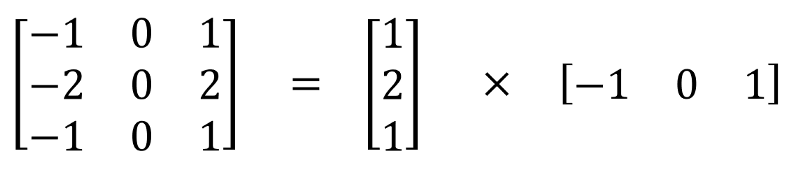
\includegraphics[width=6cm]{plots/05_conv_variations/separable/seprablematrix.png}
         \caption{In convolution, the 3x3 kernel directly convolves with the image. In spatially separable convolution, the 3x1 kernel first convolves with the image. Then the 1x3 kernel is applied. This would require 6 instead of 9 parameters while doing the same operations.}
     \end{figure}
     \end{itemize}
 \end{vbframe}
%%%%%%%%%%%%%%%%%%%%%%%%%%%%%%%%%%%%%%%%

\begin{vbframe}{Spatially separable convolution}
  
  Example 1: A convolution on a $5 \times 5$ image with a $3 \times 3$ kernel (stride=1, padding=0) requires scanning the kernel at 3 positions horizontally and 3 vertically. That is 9 positions in total, indicated as the dots in the image below. At each position, 9 element-wise multiplications are applied. Overall, that is 9 x 9 = 81 multiplications.
     \begin{figure}
         \centering
         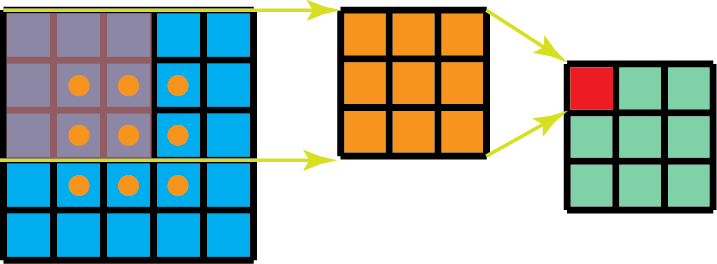
\includegraphics[width=4cm]{plots/05_conv_variations/separable/sep0.png}
         \caption{Standard convolution with 1 channel.}
     \end{figure}
   
     \begin{figure}
         \centering
         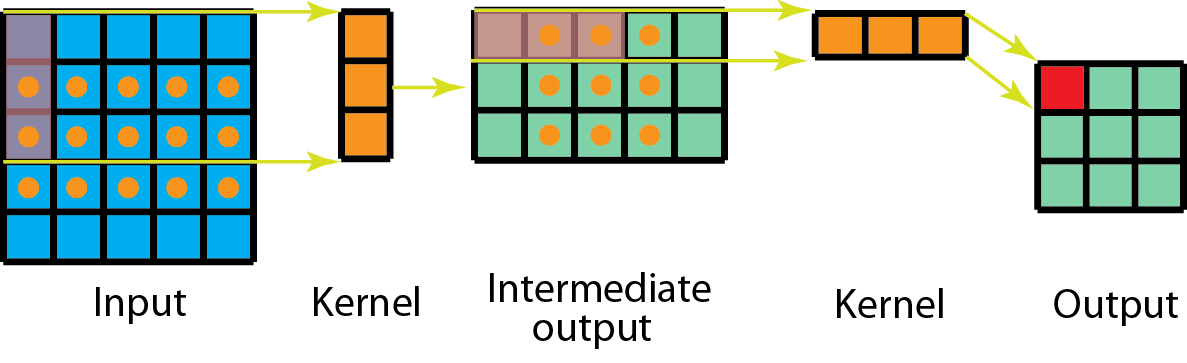
\includegraphics[width=8cm]{plots/05_conv_variations/separable/sep1.png}
         \caption{Spatially separable convolution with 1 channel. Overall, the spatially separable convolution takes 45 + 27 = 72 multiplications. (Image source: Bai (2019))}
     \end{figure}
     
    

   \textbf{Note:} However, despite their advantages, spatial separable convolutions are seldom applied in deep learning. This is mainly due to not all kernels being able to get divided into two smaller ones. Replacing all standard convolutions by spatial separable would also introduce a limit in searching for all possible kernels in the training process, implying worse training results.
   
\end{vbframe}
%%%%%%%%%%%%%%%%%%%%%%%%%%%%%%%%%%%%%%%%

\begin{vbframe}{Depthwise separable convolution}
   \begin{itemize}
     \item The depthwise separable convolutions, which is much more commonly used in deep learning (e.g. in MobileNet and Xception).
     \item This convolution separates convolutional process into two stages of depthwise and pointwise.
   \end{itemize}

 
\begin{figure}
\centering
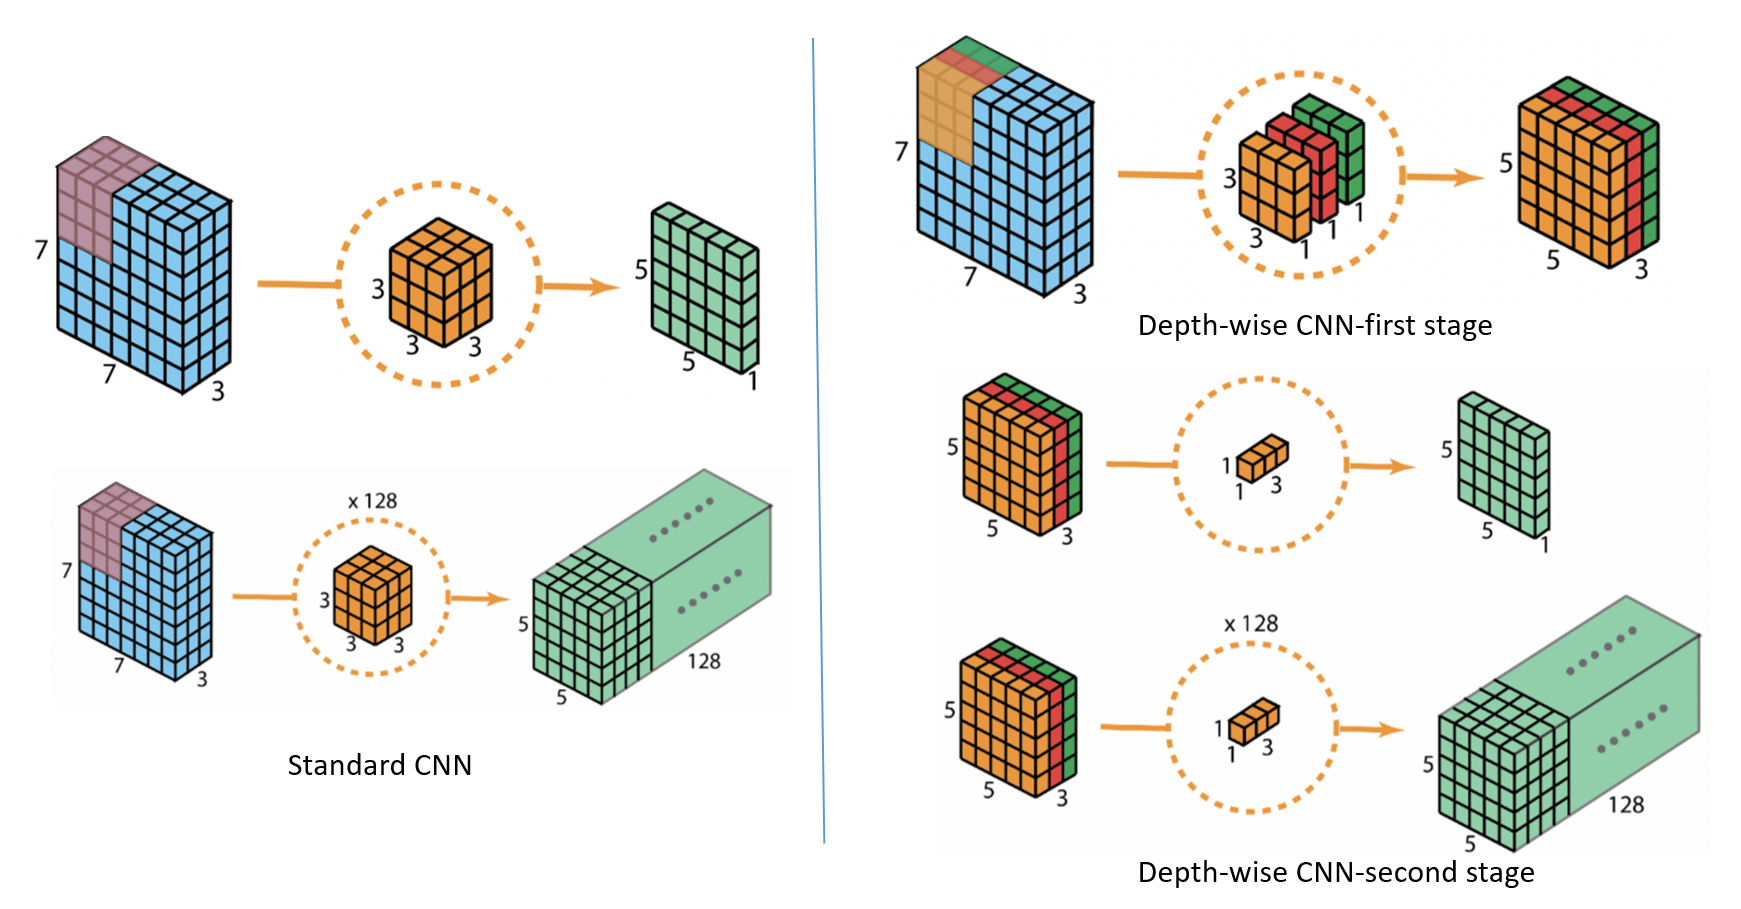
\includegraphics[width=8cm]{plots/05_conv_variations/separable/Depthwise.png}
\caption{Comparison between standard cnn and separable depthwise cnn}
\end{figure}
     
     
\begin{figure}
\centering
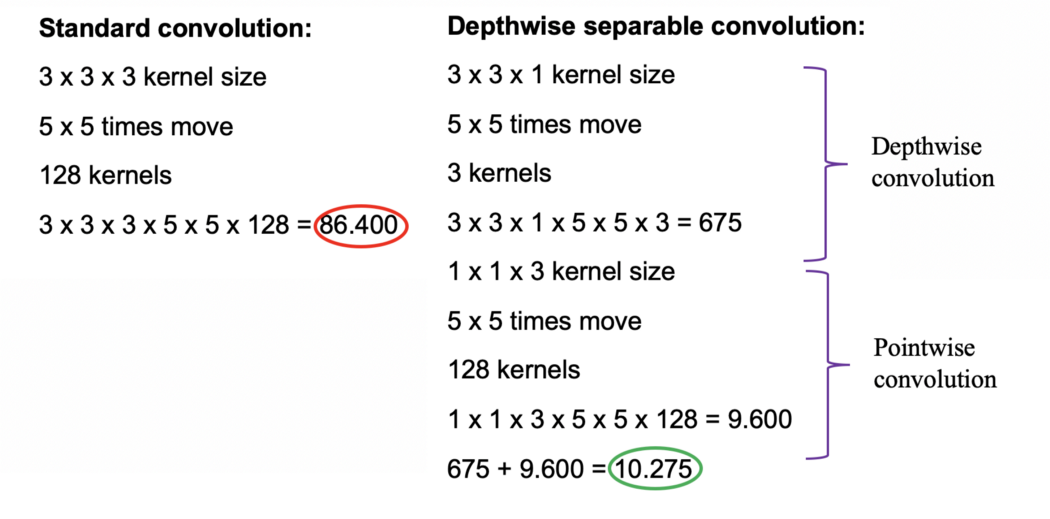
\includegraphics[width=9cm]{plots/05_conv_variations/separable/example-depthwise2.png}
\caption{Comparision of number of multiplications in Depthwise separable cnn and standard cnn}
\end{figure}
     
Therefore, fewer computations leads faster network.
     
\begin{figure}
\centering
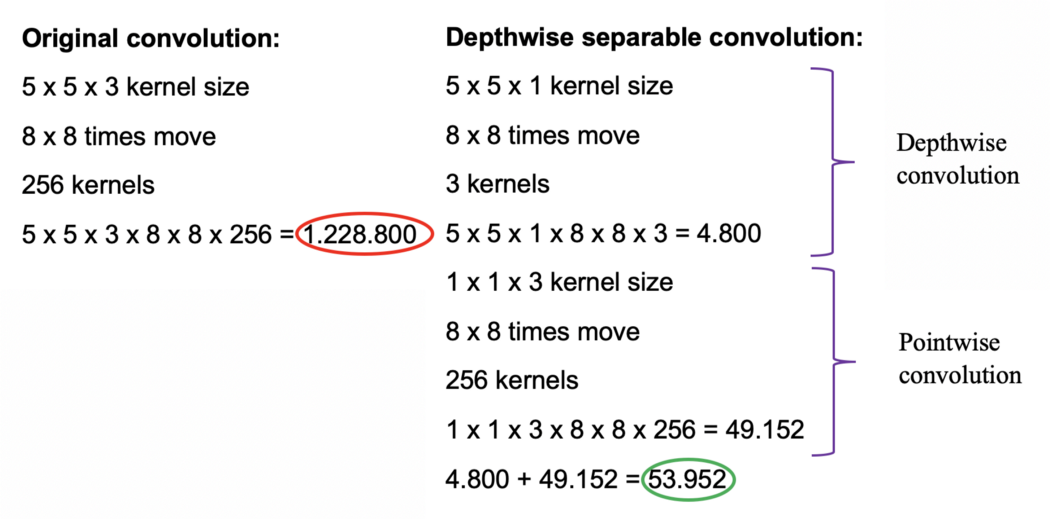
\includegraphics[width=9cm]{plots/05_conv_variations/separable/example-depthwise1.png}
\caption{Comparision of number of multiplications in Depthwise separable cnn and standard cnn}
\end{figure}
     
\end{vbframe}
%%%%%%%%%%%%%%%%%%%%%%%%%%%%%%%%%%%%%%%%

\begin{vbframe}{Depthwise convolution }
 
 As the name suggests, we perform kernel on depth of the input volume (on the input channels). The steps followed in this convolution are:

   \begin{itemize}
     \item Take number of kernels equal to the number of input channels, each kernel having depth 1. Example, if we have a kernel of size $3\times 3$ and an input of size $6\times 6$ with 16 channels, then there will be $16 \times 3 \times 3$ kernels.
     \item Every channel thus has 1 kernel associated with it. This kernel is convolved over the associated channel separately resulting in 16 feature maps.
     \item Stack all these feature maps to get the output volume with $4 \times 4$ output size and 16 channels.
   \end{itemize}

     
\end{vbframe}
%%%%%%%%%%%%%%%%%%%%%%%%%%%%%%%%%%%%%%%

\begin{vbframe}{Pointwise convolution }
 
As the name suggests, this type of convolution is applied to every single point in the convolution separately (remember $1\times 1$ convs?). So how does this work?

   \begin{itemize}
     \item Take a $1\times 1$ conv with number of filters equal to number of channels you want as output.
     \item Perform basic convolution applied in $1\times 1$ conv to the output of the Depth-wise convolution.
   \end{itemize}

     
\end{vbframe}
%%%%%%%%%%%%%%%%%%%%%%%%%%%%%%%%%%%%%%%%%

\section{Flattening}

\begin{vbframe}{Flattening}
    
Flattening is converting the data into a 1-dimensional array for inputting it to the next layer. We flatten the output of the convolutional layers to create a single long feature vector. And it is connected to the final classification model, which is called a fully-connected layer.
          
\begin{figure}
\centering
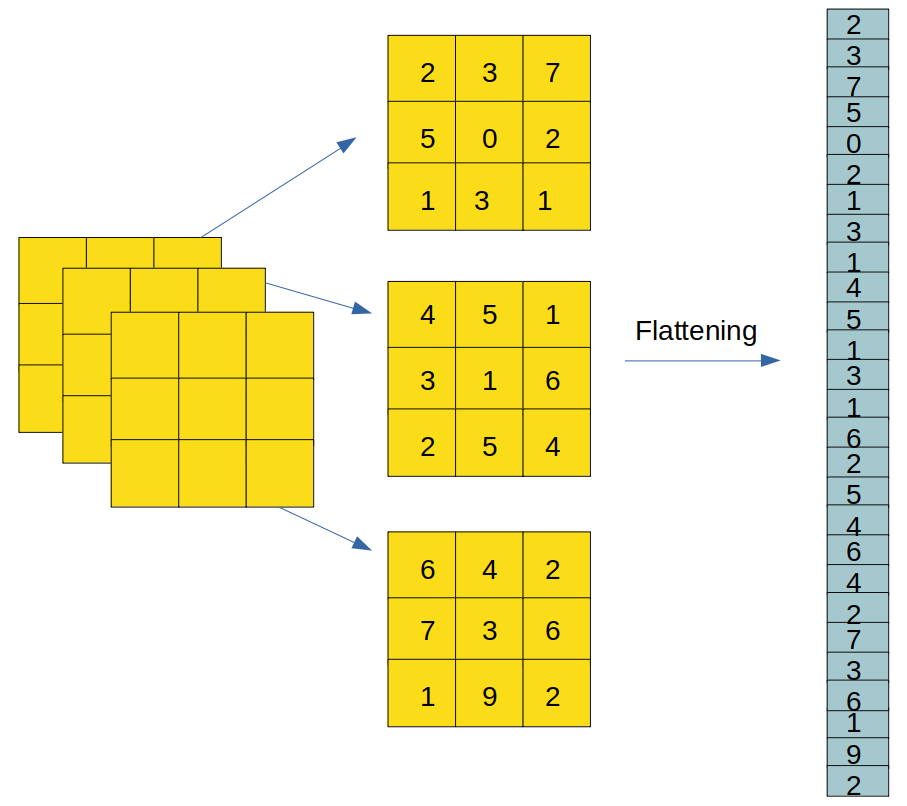
\includegraphics[width=6cm]{figure/flatten.png}
\end{figure}

\end{vbframe}



%%%%%%%%%%%%%%%%%%%%%%%%%%%%%%%%%%%%%%%%%%%%%%%%%%%%%%%%%%%%%%%%%%
%%%%%%%%%%%%%%%%%%%%%%%%%%%%%%%%%%%%%%%%%%%%%%%%%%%%%%%%%%%%%%%%%%
%%%%%%%%%%%%%%%%%%          REFERENCES          %%%%%%%%%%%%%%%%%%
%%%%%%%%%%%%%%%%%%%%%%%%%%%%%%%%%%%%%%%%%%%%%%%%%%%%%%%%%%%%%%%%%%
\begin{vbframe}
\frametitle{References}
\footnotesize{
\begin{thebibliography}{99}

\bibitem[Dumoulin et al., 2016]{14} Dumoulin, Vincent and Visin, Francesco (2016)
\newblock A guide to convolution arithmetic for deep learning
\newblock \emph{\url{https://arxiv.org/abs/1603.07285v1}}
%%%%%%%%%%%%%%%%%%%%%%%%%%%%%%%%%%
\bibitem[van den Oord et al., 2016]{15} Van den Oord, Aaron, Sander Dielman, Karen Simonyan, Oriol Vinyals, Alex Graves, Nal Kalchbrenner, and Koray Kavukocuoglu (2016)
\newblock WaveNet: A Generative Model for Raw Audio
\newblock \emph{\url{https://arxiv.org/abs/1609.03499}}
%%%%%%%%%%%%%%%%%%%%%%%%%%%%%%%%%%
%%%%%%%%%%%%%%%%%%%%%%%%%%%%%%%%%%
\bibitem[Gennart et al., 1996]{17} Benoit A., Gennart, Bernard Krummenacher, Roger D. Hersch, Bernard Saugy, J.C. Hadorn and D. Mueller (1996)
\newblock The Giga View Multiprocessor Multidisk Image Server
\newblock \emph{\url{https://www.researchgate.net/publication/220060811_The_Giga_View_Multiprocessor_Multidisk_Image_Server}}
%%%%%%%%%%%%%%%%%%%%%%%%%%%%%%%%%%
%%%%%%%%%%%%%%%%%%%%%%%%%%%%%%%%%%
\bibitem[Tran et al., 2015]{18} Tran, Du, Lubomir Bourdev, Rob Fergus,  Lorenzo Torresani and Paluri Manohar (2015)
\newblock Learning Spatiotemporal Features with 3D Convolutional Networks
\newblock \emph{\url{https://arxiv.org/pdf/1412.0767.pdf}}
%%%%%%%%%%%%%%%%%%%%%%%%%%%%%%%%%%
%%%%%%%%%%%%%%%%%%%%%%%%%%%%%%%%%%
\bibitem[Milletari et al., 2016]{19} Milletari, Fausto, Nassir Navab and  Seyed-Ahmad Ahmadi (2016)
\newblock V-Net: Fully Convolutional Neural Networks for
Volumetric Medical Image Segmentation
\newblock \emph{\url{https://arxiv.org/pdf/1606.04797.pdf}}
%%%%%%%%%%%%%%%%%%%%%%%%%%%%%%%%%%
%%%%%%%%%%%%%%%%%%%%%%%%%%%%%%%%%%
\bibitem[Zhang et al., 2015]{20} Zhang, Xiang, Junbo Zhao and Yann LeCun (2015)
\newblock Character-level Convolutional Networks for Text Classification
\newblock \emph{\url{http://arxiv.org/abs/1509.01626}}
%%%%%%%%%%%%%%%%%%%%%%%%%%%%%%%%%%
%%%%%%%%%%%%%%%%%%%%%%%%%%%%%%%%%%
\bibitem[Wang et al., 2017]{21} Wang, Zhiguang, Weizhong Yan and Tim Oates (2017)
\newblock Time Series Classification from Scratch with Deep Neural Networks: A Strong Baseline
\newblock \emph{\url{http://arxiv.org/abs/1509.01626}}
%%%%%%%%%%%%%%%%%%%%%%%%%%%%%%%%%%
%%%%%%%%%%%%%%%%%%%%%%%%%%%%%%%%%%
\bibitem[Yu et. al, 2015]{22} Fisher Yu and Vladlen Koltun (2015)
\newblock Multi-Scale Context Aggregation by Dilated Convolutions
\newblock \emph{\url{https://arxiv.org/abs/1511.07122}}
%%%%%%%%%%%%%%%%%%%%%%%%%%%%%%%%%%
%%%%%%%%%%%%%%%%%%%%%%%%%%%%%%%%%%
\bibitem[Bai et. al, 2018]{23} Bai, Shaojie,  Zico J. Kolter and Vladlen Koltun (2018)
\newblock An Empirical Evaluation of Generic Convolutional and Recurrent Networks for Sequence Modeling
\newblock \emph{\url{http://arxiv.org/abs/1509.01626}}
%%%%%%%%%%%%%%%%%%%%%%%%%%%%%%%%%%
%%%%%%%%%%%%%%%%%%%%%%%%%%%%%%%%%%
\bibitem[Odena et. al , 2017]{24} Augustus Odena, Vincent Dumoulin and Chris Olah (2016)
\newblock Deconvolution and Checkerboard Artifacts
\newblock \emph{\url{https://distill.pub/2016/deconv-checkerboard/}{https://distill.pub/2016/deconv-checkerboard/}}
%%%%%%%%%%%%%%%%%%%%%%%%%%%%%%%%%%
%%%%%%%%%%%%%%%%%%%%%%%%%%%%%%%%%%
\bibitem[Arauho et. al , 2019]{45} Andre Araujo, Wade Norris and Jack Sim (2019)
\newblock Computing Receptive Fields of Convolutional Neural Networks
\newblock \emph{\url{https://distill.pub/2019/computing-receptive-fields/}}
%%%%%%%%%%%%%%%%%%%%%%%%%%%%%%%%%%
%%%%%%%%%%%%%%%%%%%%%%%%%%%%%%%%%%
\bibitem[Wang et. al , 2017]{31} Zhiguang Wang, Yan, Weizhong and Tim Oates (2017)
\newblock Time series classification from scratch with deep neural networks: A
strong baseline
\newblock \emph{\url{https://arxiv.org/1611.06455}}
%%%%%%%%%%%%%%%%%%%%%%%%%%%%%%%%%%
%%%%%%%%%%%%%%%%%%%%%%%%%%%%%%%%%%
\bibitem[Lin et al., 2017]{38} Lin, Haoning and Shi, Zhenwei and Zou, Zhengxia (2017)
\newblock Maritime Semantic Labeling of Optical Remote Sensing Images with Multi-Scale Fully Convolutional Network

\end{thebibliography}
}
\end{vbframe}




\endlecture
\end{document}